\documentclass[11pt,a4paper]{article}
\usepackage[hyperref]{emnlp2020}
\usepackage{times}
\usepackage{latexsym}
\usepackage{graphicx}
\renewcommand{\UrlFont}{\ttfamily\small}

\usepackage{microtype}

\aclfinalcopy % Uncomment this line for the final submission

\newcommand\BibTeX{B\textsc{ib}\TeX}

\title{A Linguistic Evaluation of Machine-Generated ``Real'' and ``Fake'' News}

\author{Aziza Mirsaidova \qquad Grace LeFevre\\
    \\
  CS 397 Seminar in Statistical Language Modeling\\
  June 10, 2022 \\}

\begin{document}
\maketitle
\begin{abstract}
Research on machine-generated fake news has often equated these two qualities, treating the task of identifying ``machine-generated'' news as equivalent to the task of identifying ``fake news.'' In this project, we create datasets of machine-generated ``real news'' and machine-generated ``fake news'' by using GPT-Neo \citep{gpt-neo} to perform text generation on input from the LIAR dataset \citep{wang2017liar}. We have two goals: 1) to assess whether this approach is an effective way to create comparable machine-generated real and fake news, and 2) to ascertain if there are any detectable stylometric or linguistic differences between real and fake news generated in this way. 
\end{abstract}

\section{Introduction}
The proliferation of fake news online has become a major concern in recent years. In particular, developments in neural language models have raised concern about machine-generated fake news being automatically disseminated on a large scale. For instance, Grover, a model for both generation and detection of fake news, successfully produced fake news rated more trustworthy than human-generated fake news \citep{zellers2019defending}. More generally, the release of any powerful language models with the ability to produce human-like text, like GPT-3, comes with the potential risk of boosting the spread of fake news and disinformation \citep{floridi2020gpt}.

Because of this risk, substantial attention has been paid to the linguistic features that might distinguish machine-generated news from human-generated news, but an underlying assumption of most work in this area has been equating ``machine-generated news'' with ``fake news." Though a significant portion of machine-generated news is fake, automated text generation techniques have also been used regularly in authentic journalism throughout the past decade, for applications like producing stories from structured datasets \citep{lecompte_2015}. More recently, work has also been done to explore how AI techniques can contribute to even more difficult news-related tasks like investigative journalism \citep{stray2019making}. With this in mind, treating ``machine-generated news detection'' and ``fake-news detection'' as equivalent tasks is clearly an oversimplification.

This project seeks to fill a specific gap in this area: investigating stylometric or linguistic differences between machine-generated fake news and machine-generated real news. In one of the few projects that explored this question, \citet{schuster2020limitations} extended otherwise truthful human-generated news stories with machine-generated additions and analyzed whether stylometry could distinguish if the augmented stories were true or false. They concluded that, while stylometry can help distinguish between human-written and machine-written text, it was not useful for differentiating true and false machine-generated text. However, since the news \citet{schuster2020limitations} analyzed was mostly human-written, with machine-generated modifications or additions comprising only a small portion of the data, it remains unclear whether there are detectable stylistic differences between primarily machine-generated real news articles and primarily machine-generated fake news articles. 

In this project, we explore this question by constructing a dataset of machine-generated real news and machine-generated fake news. We take sentences from the LIAR dataset \citep{wang2017liar} that were rated true and false as input to generate paragraphs of text using GPT-Neo. This process yields two sets of data, one machine-generated ``fake news'' data set and one machine-generated ``real news'' data set. We compare the two sets of articles using several linguistic features, including: named entities, referential words, and Zipf distributions. Lastly, we use classification methods to predict whether the news articles we generated are real or fake news. We have two broad in this process. First, we want to assess whether our data generation strategy is a useful way to create datasets of machine-generated ``real'' and ``fake'' news. Second, we want to determine whether linguistic features can help in distinguishing real news articles and fake news articles that are both machine-generated by the same model. 

\section{Data Generation}
\subsection{The LIAR Dataset}
LIAR \citep{wang2017liar} is a publicly available dataset for fake news detection. It consists of 12.8K human-labeled short statements occurring in various contexts collected from \url{politifact.com}. Based on the evaluation and justification of a \url{politifact.com} editor, each statement is labeled for truthfulness with one of six fine-grained ratings: pants on fire, false, barely true, half true, mostly true, and true. For the purposes of this project, we are only interested in the sentences labeled ``false'' and ``true.'' Figure \ref{fig:LIAR_example} shows an example of a false statement from the LIAR dataset. 

\subsection{Text Generation Process}
We performed text generation using GPT-Neo 1.3B, a pre-trained transformer model designed using EleutherAI's replication of the GPT-3 architecture \citep{gpt-neo}. GPT-Neo 1.3B was trained on the Pile dataset \citep{gao2020pile} for 380B tokens over 362,000 steps as a masked autoregressive language model using cross-entropy loss. This model is useful for our purposes because it was pretrained for generating texts from a prompt. 

From the LIAR training dataset, we extracted the first 1000 true statements and the first 1000 false statements. Each true and false statement collected in this way was fed to this GPT-Neo model as a prompt for text generation. After experimenting with different parameter values, we settled on the following ones: max\_length = 200, do\_sample = True, temperature = 0.9, top\_k = 50. This process yielded a paragraph of text for each statement, for a total of 1000 ``fake news'' paragraphs and 1000 ``real news'' paragraphs. An example of each is shown in Figure \ref{fig:generated_examples}. 

\begin{figure}
    \centering
    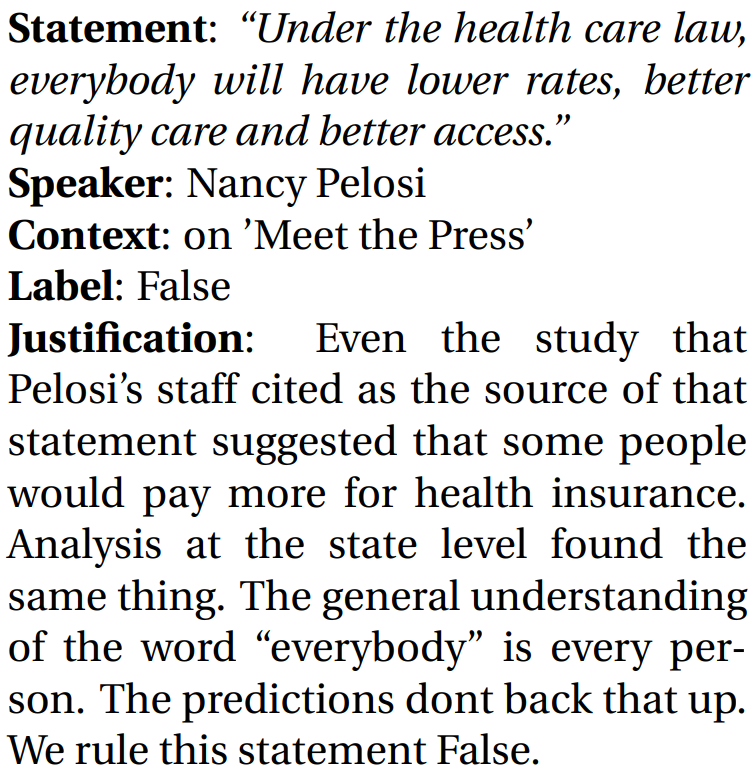
\includegraphics[width=6cm]{LIARexample.png}
    \caption{Example statement from LIAR data \citep{wang2017liar}}
    \label{fig:LIAR_example}
\end{figure}

\begin{figure}
    \centering
    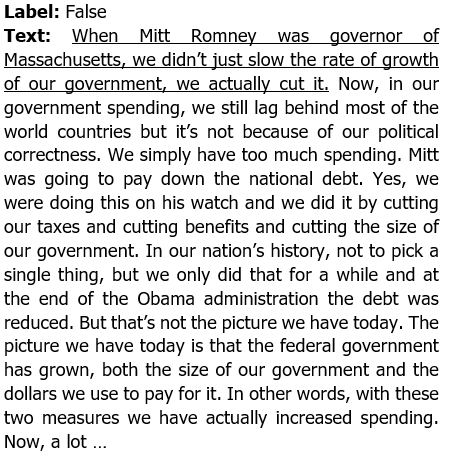
\includegraphics[width=7cm]{emnlp2020-templates/generated_example_false.png}
    \par\noindent\rule[1pt]{7cm}{0.4pt}
    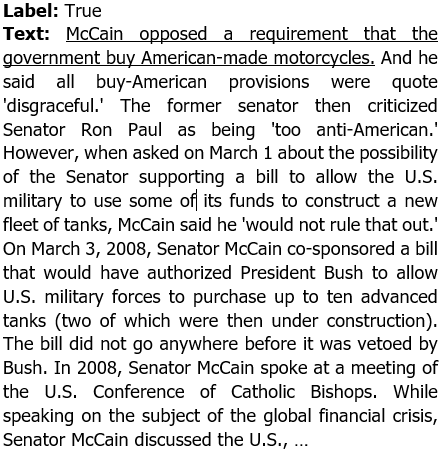
\includegraphics[width=7cm]{emnlp2020-templates/generated_example_true.png}
    \caption{Example ``false'' and ``true'' paragraphs from our generated data. The underlined sentence is the text that was provided as a prompt and the remainder was generated with GPT-Neo}
    \label{fig:generated_examples}
\end{figure}

\subsection{Discussion}
It's important to note a couple limitations of our data generation process. One limitation is that, since we specified a set sequence length, the paragraphs do not always end in a complete sentence. This is clearly not how paragraphs from human-generated real or fake news would be. Another important note is that, even though our ``real'' news examples were generated from statements rated ``true'' in the LIAR dataset, there is no guarantee that all of the information in the generated ``true'' paragraphs is actually true. For these and other reasons, we do not claim that our dataset consists of actual real and fake news but rather that it serves as a proxy for real and fake machine-generated news in the form of machine-generated text based on true or false input statements.

\section{Linguistic Feature Analysis}
We performed several types of linguistic feature analyses to compare our ``real news'' and ``fake news'' datasets, detailed below. 

\subsection{Named Entity Recognition}
 Named Entity Recognition (NER) is a widely used NLP technique that seeks to locate and classify named entities in a given text into pre-defined categories including person names, organizations, locations, quantities, expression of times, monetary values, etc. With the use of NER, we can extract main entities in a text which helps to sort unstructured data and detect important information from text. Prior to applying NER method to our dataset, we utilized NLTK's sentence tokenizer and removed special characters. 
 
 \begin{figure}
    \centering
    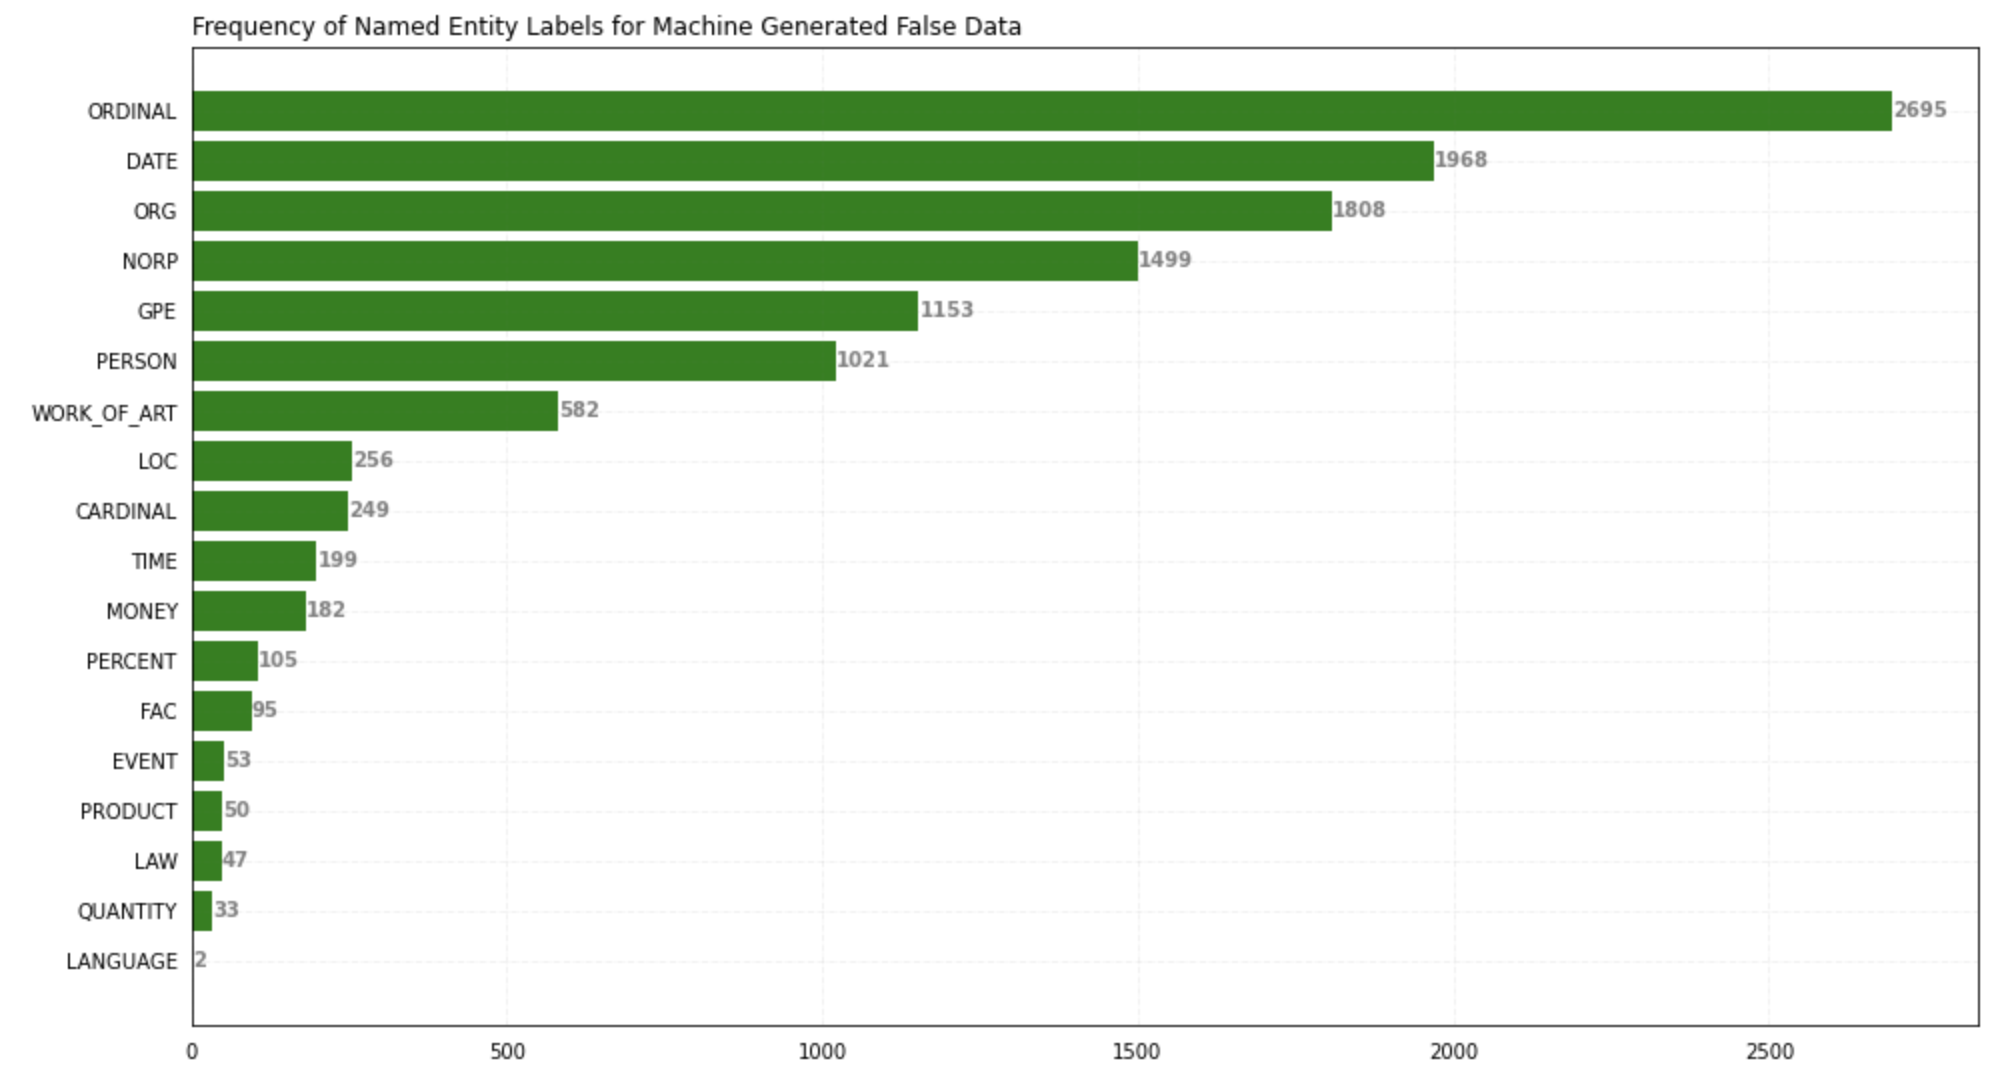
\includegraphics[width=7.5cm]{emnlp2020-templates/False NER.png}
    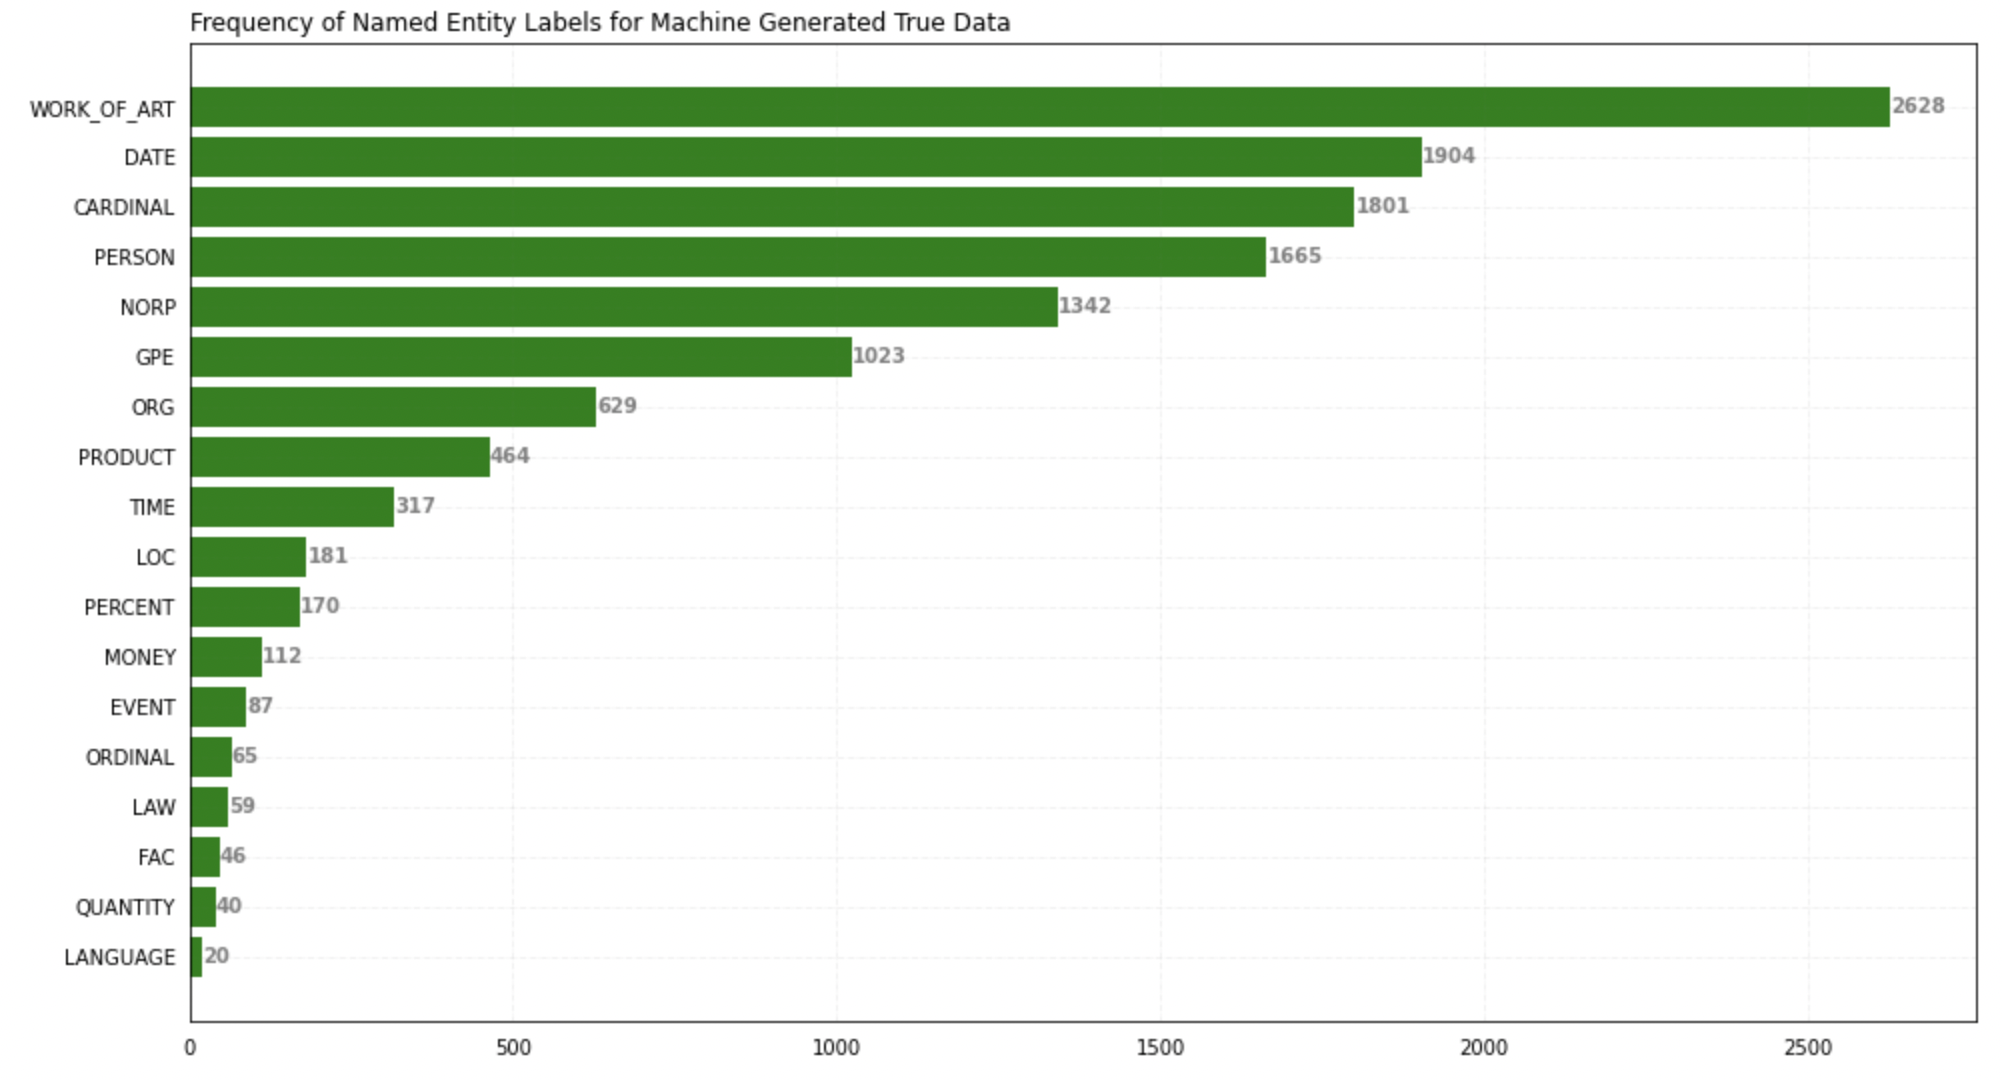
\includegraphics[width=7.5cm]{emnlp2020-templates/True NER.png}
    \caption{Named Entity Recognition distribution for unique occurrences of entities in ``false'' and ``true'' datasets.}
    \label{fig:NER}
\end{figure}
 
 Spacy's Entity Recognizer pipeline assisted us in extracting entities from machine generated text. We found that there are 11,997 entities consisting of 16 unique entity labels in the false dataset, as shown in the upper bar chart in Figure \ref{fig:NER}. The total number of entities in the true dataset exceeded this, with 12,553 entities, as shown in the lower bar chart in Figure \ref{fig:NER}. In the fake news, ordinal, date, organization, nationalities and political groups, geopolitical and person entities are the most frequent entities with over one thousand occurrences in a sentence. The entities obtained from the true news differ somewhat from the false news with work of art, date, cardinal, person entities most frequent in the text. 
 
 These results show that entities related to both true and false news differs in accordance with type of information involved in the dataset. For example, since false news commonly highlights the numerical and time information to bring more attention, it makes sense that the ordinal and date entities are the most frequent entities in the list. Further understanding the entities in both original and machine generated news may help with recognizing the differences as well as their contribution to fake news detection.
 
\subsection{Referential words}
Frequency of referential words in a text, like pronouns and proper nouns, has been examined in the context of fake news applications to see if it is correlated with truthfulness  \citep[e.g.][]{mahyoob2020linguistic}. We used the Spacy package in Python to analyze referential term frequency by performing part of speech tagging and identifying pronouns and proper nouns. The results, as shown in Table \ref{table:ref_words}, do not suggest any significant difference between the true and false data with respect to referential terms. The frequency of both pronouns and proper nouns is slightly lower in the true data, but likely not enough to be significant.

\begin{table}
\centering
\begin{tabular}{ c||c|c } 
  & Pronouns & Proper Nouns\\ 
 \hline
 False data & 0.04713 & 0.07648 \\ 
 True data & 0.04392 & 0.07453 \\ 
\end{tabular}
\caption{Frequency of pronouns and proper nouns in ``false'' and ``true'' datasets, measured relative to all tokens present in each corpus}
\label{table:ref_words}
\end{table}

\subsection{Zipf distributions}
Zipf's Law states that, for a large enough corpus of text, the frequency with which a word is used in the corpus decreases with its rareness in the text in an approximately hyperbolic way \citep{baayen2001word}. That is, the most frequent word in a corpus will appear twice as often as the second-most frequent word in the corpus, and so forth. Human language maintains this frequency distribution in an extremely reliable way cross-linguistically \citep{piantadosi2014zipf}. As a result, checking the Zipf distribution of a corpus can be a useful way of assessing how well it approximates human language. 

Figure \ref{fig:Zipf} shows the Zipf distributions for our generated corpora, using the 100 most frequent words in each. There don't seem to be significant differences between the two plots, but neither follow the frequency distribution that would be expected of natural language. For example, it is clear that the most frequent word is about three times as frequent as the second-most frequent word. This suggests that Zipf distributions remain an excellent way of detecting machine-generated text in general, but do not lend insight into distinguishing fake machine-generated text from true machine-generated text.

\begin{figure}
    \centering
    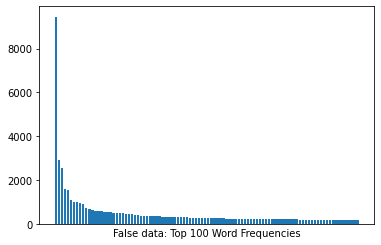
\includegraphics[width=7cm]{emnlp2020-templates/Zipf_false.png}
    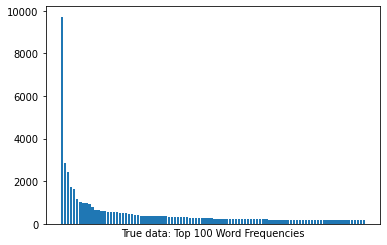
\includegraphics[width=7cm]{emnlp2020-templates/Zipf_true.png}
    \caption{Zipf distributions for our ``false'' and ``true'' datasets, using the 100 most frequent words in each}
    \label{fig:Zipf}
\end{figure}

\section{Automatic Fake News Detection}
We conducted fake news classification in our machine generated fake and true news dataset to understand performance of classification methods in machine generated text. Initially, we pre-processed the data creating a dataframe including false and true news in "text" column and binary labeled them in "labels" columns which shows whether text are representative of fake or true news. In addition, we counted the words using CountVectorizer and IDF and Tf-IDF which provides output in a sparse matrix representing the text. Then, we split the data into train and test sets training them in models shown in Figure \ref{fig:Models}.

\begin{figure}
    \centering
    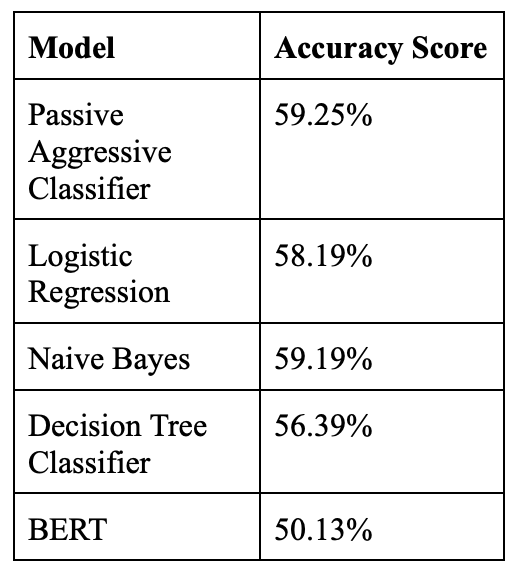
\includegraphics[width=5cm]{emnlp2020-templates/Models.png}
    \caption{Classification models and their corresponding accuracy score detects the fake news based on machine generated "true" and "false" datasets.}
    \label{fig:Models}
\end{figure}

As seen in Figure \ref{fig:Models}, Passive Aggressive Classifier exhibited the highest result in accordance with other classification techniques. It's an online learning algorithm that remains passive for correct classification outcome and aggressive to the lowest. Based on the accuracy score of the models, we can conclude that size of the dataset significantly effected the model performance to detect fake news. 

\section{Conclusion}
This project highlights the importance of distinguishing the task of detecting ``machine-generated'' news from the task of detecting ``fake news.'' In the future, we would like to extend our data generation process to create much larger machine-generated datasets and then perform more extensive linguistic feature analysis, with the goal of identifying features we could add to a discriminator model to better distinguish between machine-generated real and fake news.

\bibliographystyle{acl_natbib}
\bibliography{anthology,emnlp2020}

\end{document}